% Setup - do not change
\documentclass[11pt]{article}
\usepackage[top=0.9in, left=0.9in, bottom=0.9in, right=0.9in]{geometry} 
\usepackage{parskip}

\usepackage[english]{babel}
\usepackage[utf8]{inputenc}
\usepackage{amsmath,amsthm,amssymb,graphicx,pdfpages,lipsum,hyperref}
\usepackage[none]{hyphenat}
\usepackage{csquotes}

\setlength\parindent{0pt}
%%%%%%%%%%%%%%%%%%%%%%%%%%%%%%%%%%%%%%%%%%%%%%%%%%%%%%%%%%%%%%%%%%%
% add other packages here if required
\usepackage{caption}
\usepackage{subcaption}
\usepackage{graphicx}
\graphicspath{ {./plots/} }
\usepackage{soul}

%% Bibliography are specified in this file. You can also choose inline bib style if you want to. But make sure your citation style is consistent (and proper)
% For more details on citation: https://library.unimelb.edu.au/recite
\usepackage[sorting = none]{biblatex}
\bibliography{references.bib}

%%%%%%%%%%%%%%%%%%%%%%%%%%%%%%%%%%%%%%%%%%%%%%%%%%%%%%%%%%%%%%%%%%% the '%' symbol denotes comments

% Begin document creation
% DELETE THE \lipsum PLACEHOLDERS WHEN YOU BEGIN
\title{\textbf{Maximize Earning for NYC For-Hire-Vehicle Drivers} \\ by Exploring the Dynamic Pricing System}
\author{
Di Wu \\
Student ID: 1208784 \\
%% Replace the link with your github repo
% 1. Remember to escape underscore (\_) in the link.
% 2. Remember to include the commit you want to submit in the link
\href{https://github.com/MAST30034-Applied-Data-Science/mast30034-project-1-WD1120}{Github repo with commit}
}


\begin{document}
\maketitle

\section{Introduction}
% Link to a 30 min tutorial if you require revision: https://www.overleaf.com/learn/latex/Learn_LaTeX_in_30_minutes

In recent years, online taxi-hailing services such as Uber, Lyft and DiDi are becoming more and more popular. One of its main advantage over traditional taxis is that passengers can see precisely when the vehicle will arrive for pick up and how much the trip is, in advance. However, frustration can occasionally still be risen for either passengers or drivers, as in large urban areas such as New York City where the traffic is heavy, the wait time can be long due to the traffic jam on the road. 

Furthermore, these service providers leverage dynamic pricing systems which change the price dynamically based on multiple factors. How could drivers optimise their day plan by taking advantage of this system that not only maximizes their income but potentially also decreases the wait time to increase satisfaction for both sides, is the research goal of this paper. 

With the supply of sufficient data, two machine learning models will be presented to explore the complex relationships between multiple features. The model's outcome and recommendation would benefit all FHV drivers. 


\section{Preprocessing}

A number of data preprocessing steps were performed on both datasets described below to ensure a consistent structure for model training. This section outlines what has been done and the expected structure of each dataset. 

\subsection{Dataset}

\subsubsection{High-Volume For-Hire-Vehicle (FHV)}
The analysis is mainly based on the FHV trip records dataset provided by the NYC Taxi \& Limousine Commission \cite{NYCTLC}, which contains comprehensive information on FHV trips within NYC, such as pickup and drop-off location and time, request time, trip distance, driver pay, additional fees, accessibility etc. It is assisted by a geometry file on taxi zones which divides NYC into 263 regions (zones) so that visualisation of the pickup and drop-off location of each trip is possible. As the research will serve future FHV drivers (2023 fall onward), it is chosen to use post-COVID data from January to December 2022 as the training data, because COVID significantly changed the way people work and entertain which dramatically affects the traffic flow. Data from January to March 2023 is used for evaluating model performance.  

\subsubsection{Primary Land Use Tax Lot Output (PLUTO)}
An additional dataset PLUTO from NYC Open Data \cite{nycPLUTO} is being used to accommodate the research goal. It contains comprehensive information on the buildings in the NYC region, including purpose, census, number of floors, floor area breakdown etc. The geographical link between the city structure and traffic flow is expected to be strong which is highly related to pick-up and drop-off demand at each location. 


\subsection{Feature Engineering}
Dimensions of the raw datasets are described in Table \ref{dataset size}. 
\begin{table}[h!]
\centering
    \begin{tabular} {|c||c|c|}
    \hline
    \textbf{Dataset} & \textbf{Records} & \textbf{Features} \\
    \hline
    TLC For-Hire Vehicle (2022) & 212,416,083 & 24 \\
    \hline
    Primary Land Use Tax Lot Output & 859,068 & 90 \\
    \hline
    \end{tabular}
    \caption{Raw dataset sizes}
    \label{dataset size}
\end{table}

A number of features have been created by aggregating other features, while some have been dropped to accommodate the research goal, and allow more intuitive analysis to be performed. By column aggregation or SQL querying, the following features from the FHV trip records dataset were selected for modelling: 

\begin{minipage}{\textwidth}
    \hspace*{1.25em}
    \begin{tabular}{@{}p{5cm}p{5cm}p{5cm}@{}}
        \textbullet\ Pickup location ID &
        \textbullet\ Trip and wait time (sec) &
        \textbullet\ Pickup hour \\
        \textbullet\ price per minute &
        \textbullet\ Trip distance (miles) &
        \textbullet\ Driver's earning (\$)
    \end{tabular}
\end{minipage}

The original PLUTO dataset has much more features. However, many features are observed with a high proportion of missing values (i.e. zoning districts) and/or irrelevant to the research goal (i.e. tax lot) after investigation. All those features have been removed. The subset of features remains were those describing the functionality of the building. Study has shown that the urban planning and function layout have important implications for the journeys of the commuters \cite{trafficFlow}, which is motivating to group the PLUTO dataset according to the taxi zone regions, and calculate the proportion of buildings from each functionality class within each region. The following features were obtained: 

\begin{minipage}{\textwidth}
    \hspace*{1.25em}
    \begin{tabular}{@{}lll@{}}
        \textbullet\ Location ID &
        \textbullet\ Number of buildings &
        \textbullet\ Proportion of commercial area \\
        \textbullet\ Proportion of residential area &
        \textbullet\ Proportion of office area &
        \textbullet\ Proportion of retail area
    \end{tabular}
\end{minipage}

\subsection{Outlier Detection}
Out of the 212,416,083 records of FHV trips, it was found that some records have insensible or incorrect values for certain features. Instances which violate any of the following rules are removed, allowing the remaining to build consistent models that are not negatively affected by outliers. 

\begin{itemize} 
    \item \textbf{Waiting time should be positive}. Records with negative time are considered to be faulty. \ul{2,660,803 records were removed}. 
    \item \textbf{Trip duration should be at least 1 minute} as trips shorter than a minute's drive are assumed to be insensible because one would rather walk for such a short trip. \ul{20,592 records were removed}. 
    \item \textbf{Trip distance should be more than 0.3 miles} based on the assumption that people would tend to just walk if the destination is within 500 meters. \ul{385,874 records were removed}. 
    \item \textbf{Positive driver fare.} Records with negative fare amount are considered to be faulty. \ul{1,127,485 records were removed}. 
    \item \textbf{Pick up location should be inside the defined NYC region} to align with the focus of this research. \ul{10,625 records were removed}. 
    \item \textbf{Price per minute should be smaller than 10}, as the 0.999 quantile of pay\_per\_min is only 4.73. \ul{75,962 outliers were removed}. 
    \item \textbf{Pay per mile should be smaller than 40}, as the 0.99 quantile of pay\_per\_mule is 20.89. \ul{274,720 outliers were removed}. 
\end{itemize} 

As a result \ul{4,297,859 trip records were removed} from the FHV dataset, which consists of approximately 2.02\% of the entirety.

From the PLUTO dataset, there are records with \textbf{sum of commercial, residential, office and retail area exceeding the total building area. Those records are removed} because all those categories are just subsets of the total building area. Although the data dictionary specifically mentioned that the sum of various areas does not always equal to total building areas, to avoid extreme outliers it was decided not to allow excess. 
\ul{127,886 records were removed} from PLUTO dataset, consists 14.9\% of the entirety. 

\subsection{Aggregation}
Given the goal of the models are to predict the unit price at each location and time, individual records are not necessary to be maintained. Instead, aggregated statistics would be more representative and be used to train the models. By grouping the FHV dataset by pickup location ID and pickup hour, averaged distance, unit price, wait time and trip time are obtained.

The PLUTO dataset is joined with the aggregated FHV dataset based on pickup location ID. The location ID is removed from the feature set afterwards so that the model can generalise better by learning from the land use information. The final training data for model training consists of 6,093 aggregated instances, with the following features:  

\begin{minipage}{\textwidth}
    \hspace*{1.25em}
    \begin{tabular}{@{}lll@{}}
        \textbullet\ Pickup hour &
        \textbullet\ Average trip distance (miles) &
        \textbullet\ Average wait and trip time (sec) \\
        \textbullet\ Number of buildings &
        \textbullet\ Proportion of commercial area &
        \textbullet\ Proportion of residential area \\
        \textbullet\ Proportion of office area &
        \textbullet\ Proportion of retail area
    \end{tabular}
\end{minipage}

With the response variable \textbf{Average Price per Minute}.


\section{Analysis and Geo-spatial Visualisation}
In this section, various visualisation techniques were utilised to explore the relationships of interest and to obtain a preliminary understanding of the data. For a consistent analysis, "price per minute" is used as the unit price and is referred to accordingly.

\subsection{Time of the day}
Passengers who travel with FHV frequently may realize that the unit price of their trip is not consistent. Indeed FHV platforms such as Uber utilise dynamic pricing based on a number of variables such as demand \cite{DynamicPricing}. From Figure \ref{PD_one_day} where 5 locations were chosen randomly to plot against pickup hour for visualisation purposes, it is clear that pickup hour affects the unit price. Location 106 has the highest price range in this figure, where its peak is about \$0.92 per minute, and trough is only about \$0.71 per minute, resulting in more than 20 cents difference. 

\begin{figure}[h]
    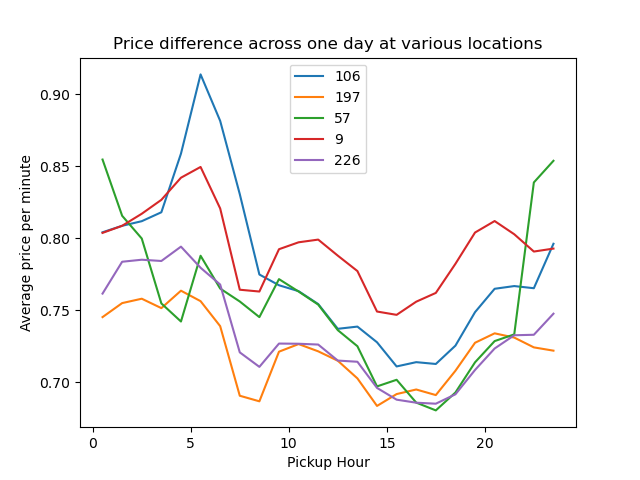
\includegraphics[width=0.55\textwidth]{plots/Price_across_one_day.png}
    \centering
    \caption{Price difference across one day}
    \label{PD_one_day}
\end{figure}

It can also be observed that the slope is different from one location to another. For example, from 7 am onwards the price raises at all locations except 106, which further declines. This could be evident that location, including the distribution characteristics of land use greatly affects the price movement. 

\subsection{Location}

\begin{figure}[h]
\centering
    \begin{minipage}{.5\textwidth}
        \centering
        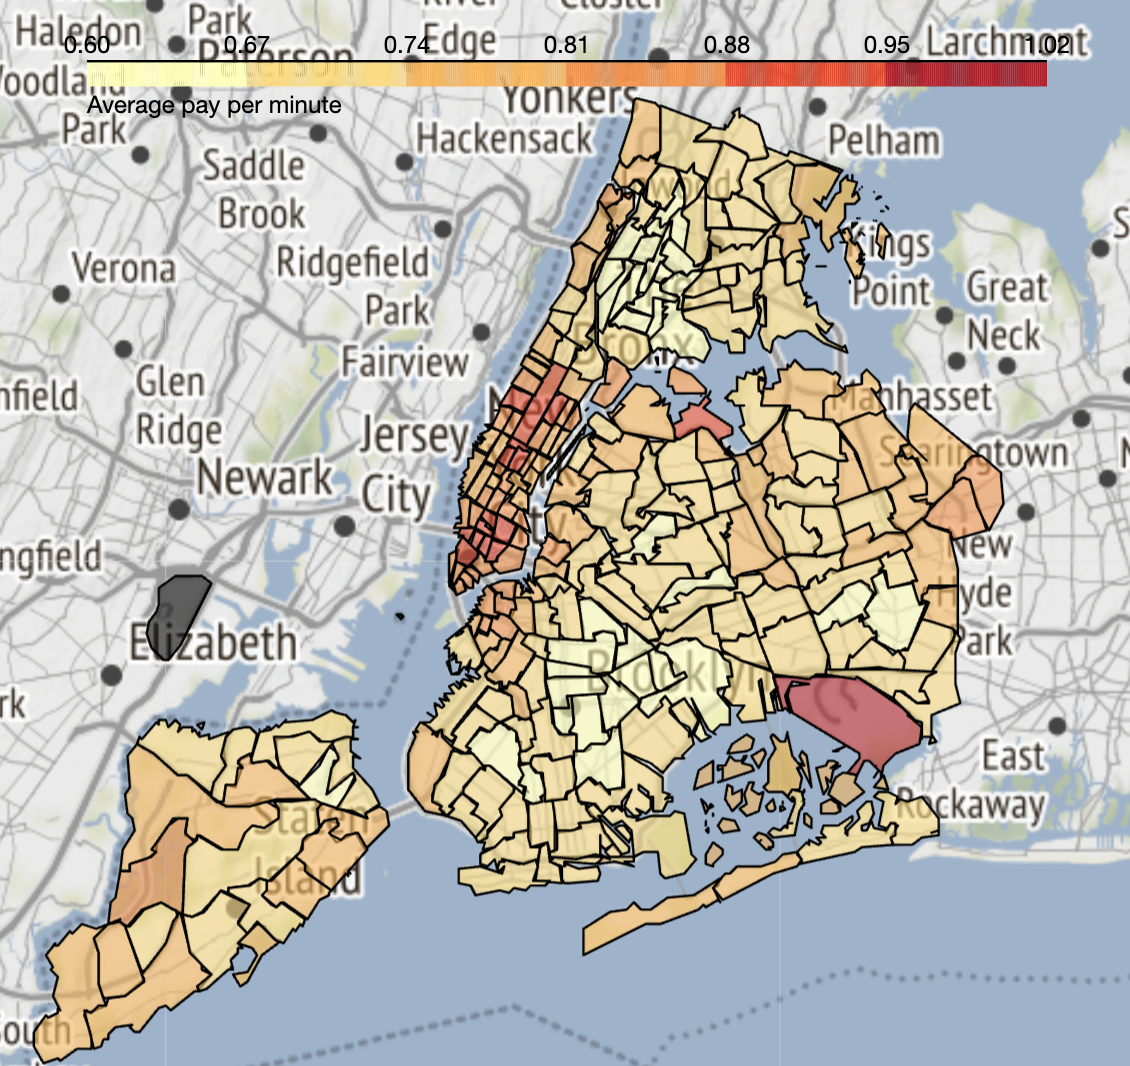
\includegraphics[width=.8\linewidth]{plots/Avg_ppmin_at8.png}
        \captionof{figure}{Average unit price at 8am}
        \label{avg_ppmin_at8}
    \end{minipage}%
    \begin{minipage}{.5\textwidth}
        \centering
        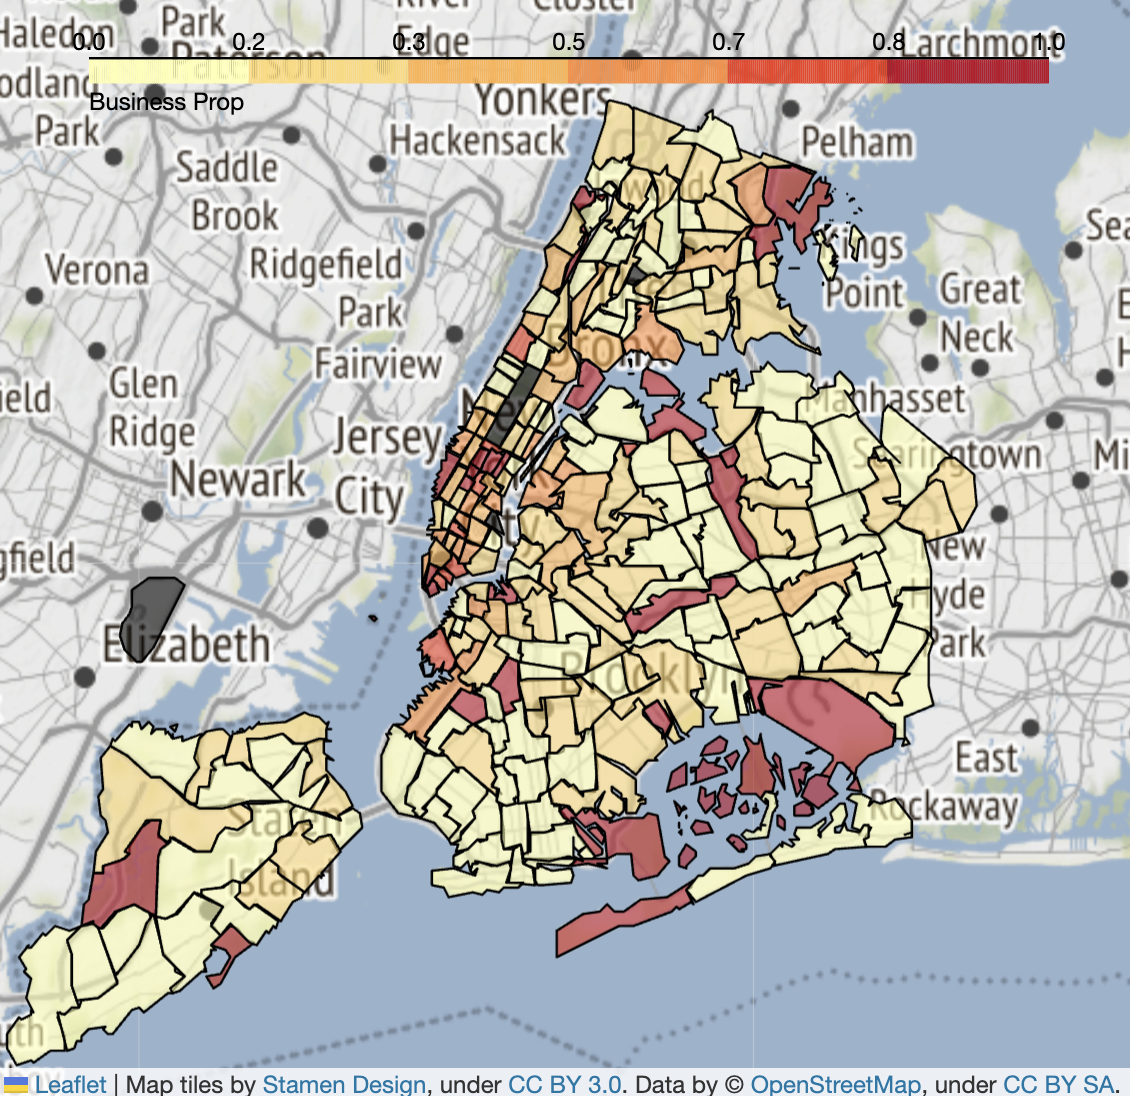
\includegraphics[width=.8\linewidth]{plots/Prop_business.png}
        \captionof{figure}{Density of non-residential area}
        \label{Prop_business}
    \end{minipage}
\end{figure}

Further investigating this relationship by capturing the average unit price of all taxi zones at a particular hour, Figure \ref{avg_ppmin_at8} shows at 8 am midtown and downtown Manhattan has the highest unit price. This is perfectly sensible as it closely matches Figure \ref{Prop_business} which shows the density of non-residential areas in each taxi zone. As one would expect, 8 am is the time people travel to get to their office and hence the CBD area would have the highest demand, leading to the highest unit price. 


\section{Modelling}
Models are trained based on the aggregated data described above, to predict the unit price of FHV trips in NYC for all taxi zones across one day. The response variable is a continuous variable, with all features being numerical except for pickup hour, which is a categorical variable. Two machine learning models: Linear Regression and Random Forest Regression are selected.

\subsection{Linear Regression}
Linear regression is one of the models capable of predicting continuous response variables based on continuous or categorical predictors. The model is trained based on the features outlined in section 2.4. As observed from Figure \ref{PD_one_day} the relationship between the unit price and pickup hour is not linear, hence pickup hour is used as a categorical variable. In addition, as the proportions of each building class sum up to less than or equal to one, they are not independent hence interaction terms are added between those 4 features. All other features are treated as numerical. 

The statistical analysis from the ordinary least squares model supports the hypothesis that all features, including the interaction terms, are significant at 0.05 significance level. 

\subsection{Random Forest Regressor}
Random forest is a combination of decision trees. Each tree contains a portion of randomly selected features, which makes the model robust to overfitting. It automatically weights all the features according to their importance with a minimum weight of 0, hence there is no need to perform feature selection in prior. In addition, unlike linear regression, random forest does not assume the relationship between features and the response variable. As a result, it is expected to fit this complex data well. 

Hyper-parameters of the model are selected by grid search. As a result, 280 decision trees are being used in the random forest regressor, with each tree selecting at most 40\% of all features, and the leaf nodes require at least 1 sample. 

\section{Discussion}
The two models built above are evaluated on the FHV trip records data between January to March 2023, which have been preprocessed and aggregated identically to the training set, as described in sections 2.2 and 2.4.

Two evaluation metrics are chosen for model comparison. $R^2$ is used as the evaluation metric for the training set, as it shows how well the data fit the regression model \cite{R_sq}. The higher it is, the better the model learns from the data. Root Mean Squared Error (RMSE) is selected as the evaluation metric for the testing set to observe how well the model generalises on unseen data, as it is an intuitive metric that measures the average difference between actual and predicted values. Based on Table \ref{Model_evaluation}, random forest regressor dominates linear regressor in both aspects.

\begin{table}[h!]
\centering
    \begin{tabular} {|c||c|c|}
    \hline
    \textbf{Model} & \textbf{$R^2$ on training set} & \textbf{RMSE on testing set} \\
    \hline
    Linear Regression & 0.709 & 0.0948 \\ 
    \hline
    Random Forest Regressor & 0.9880 & 0.0920 \\
    \hline
    \end{tabular}
    \caption{Model evaluation}
    \label{Model_evaluation}
\end{table}

\begin{figure}[h]
    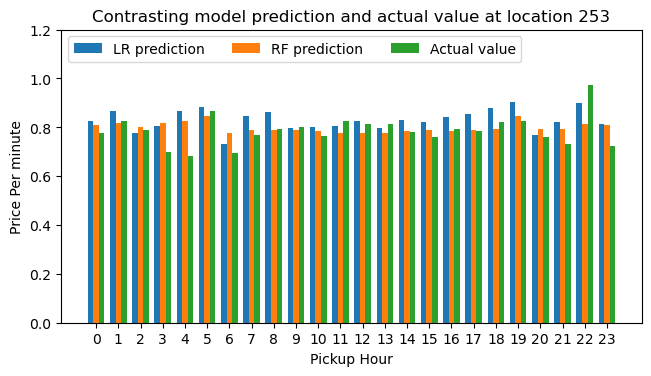
\includegraphics[width=0.7\textwidth]{plots/Pred_contrast_253.png}
    \centering
    \caption{Contrast model predictions on 'unit price' at location 253} 
    \label{contrast_pred}
\end{figure}

 Visualising the predictions made by both models and the actual value at location 253 (the location with the highest price volatility observed), Figure \ref{contrast_pred} shows that both models did actually learn from the training data pretty well. Although LR overestimates the price in most pickup hours, the discrepancy is very small in the morning hours, perhaps because of the large number of trip records available in the morning. In contrast, both models consistently overestimate the response variable at 3 am and 4 am, which can be caused by the lack of trip records during this time as expected, which makes the aggregated data not as representative as other hours. During the day, the RF model has predictions very close to the actual values which further proves the model's high performance.

\begin{figure}[h]
    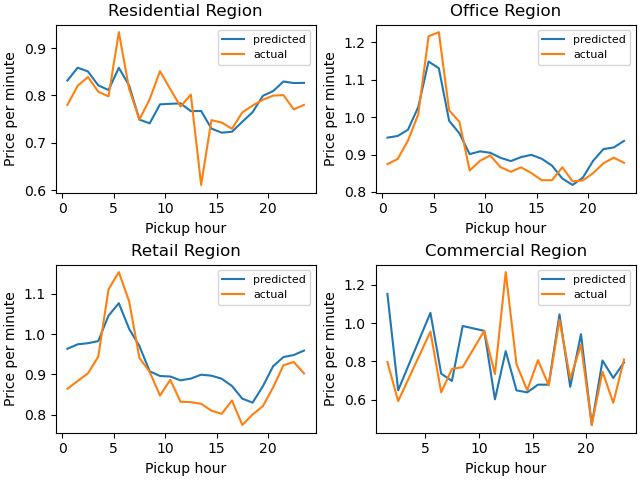
\includegraphics[width=0.7\textwidth]{plots/contrast_by_loc.png}
    \centering
    \caption{Contrast model predictions on representative locations}
    \label{contrast_loc}
\end{figure}

Recall that the research goal is finding out the optimal strategy for FHV drivers to maximise their earnings. In order to explore the relationship between price and land use, the most representative  locations which have the highest proportion of commercial, residential, office and retail are chosen. From Figure \ref{contrast_loc} it is observed that the price movement in different regions has different characteristics, which the model demonstrates the ability to capture. Although the predicted values do not fully align with the actual value, the slope matches well which is evident that the model generalises. 

A pickup hour of interest is 6 am - the global maximum of residential, office, and retail dominated regions, where the model underestimates. The prediction of unit price made by the RF model as shown in \ref{RFpred6} indicates that most locations with the highest fare are in Manhattan. The unit price in the region can reach above \$1 according to Figure \ref{contrast_loc}, and it is indeed dominated by office and retail areas. The error between the predicted and actual values as shown in Figure \ref{RFerror6} centres around 0, with a few locations underestimated and a few overestimated. Overall no systematic bias has been detected. 

\begin{figure}[h]
\centering
    \begin{minipage}{.5\textwidth}
        \centering
        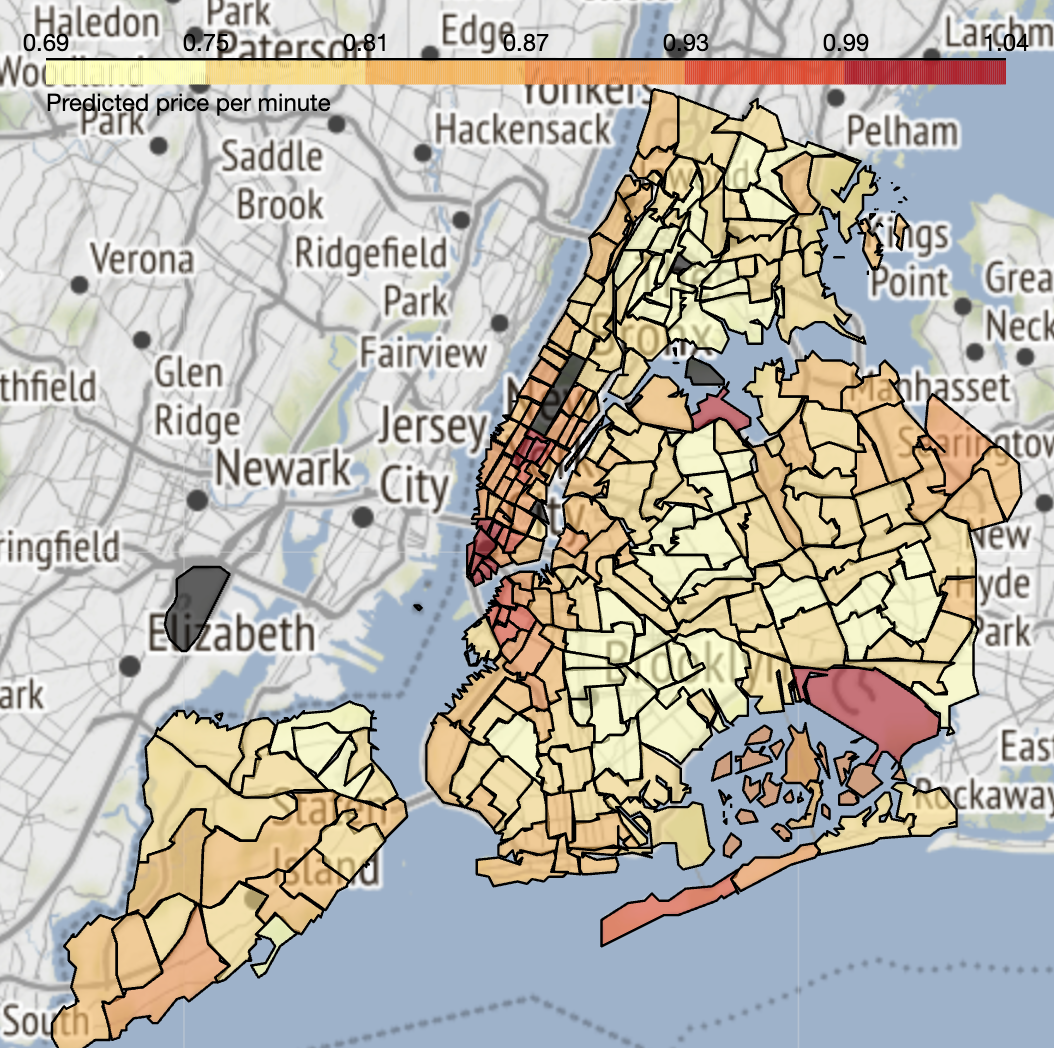
\includegraphics[width=.94\linewidth]{plots/RFpred_6am.png}
        \captionof{figure}{RF prediction of unit price at 6 am}
        \label{RFpred6}
    \end{minipage}%
    \begin{minipage}{.5\textwidth}
        \centering
        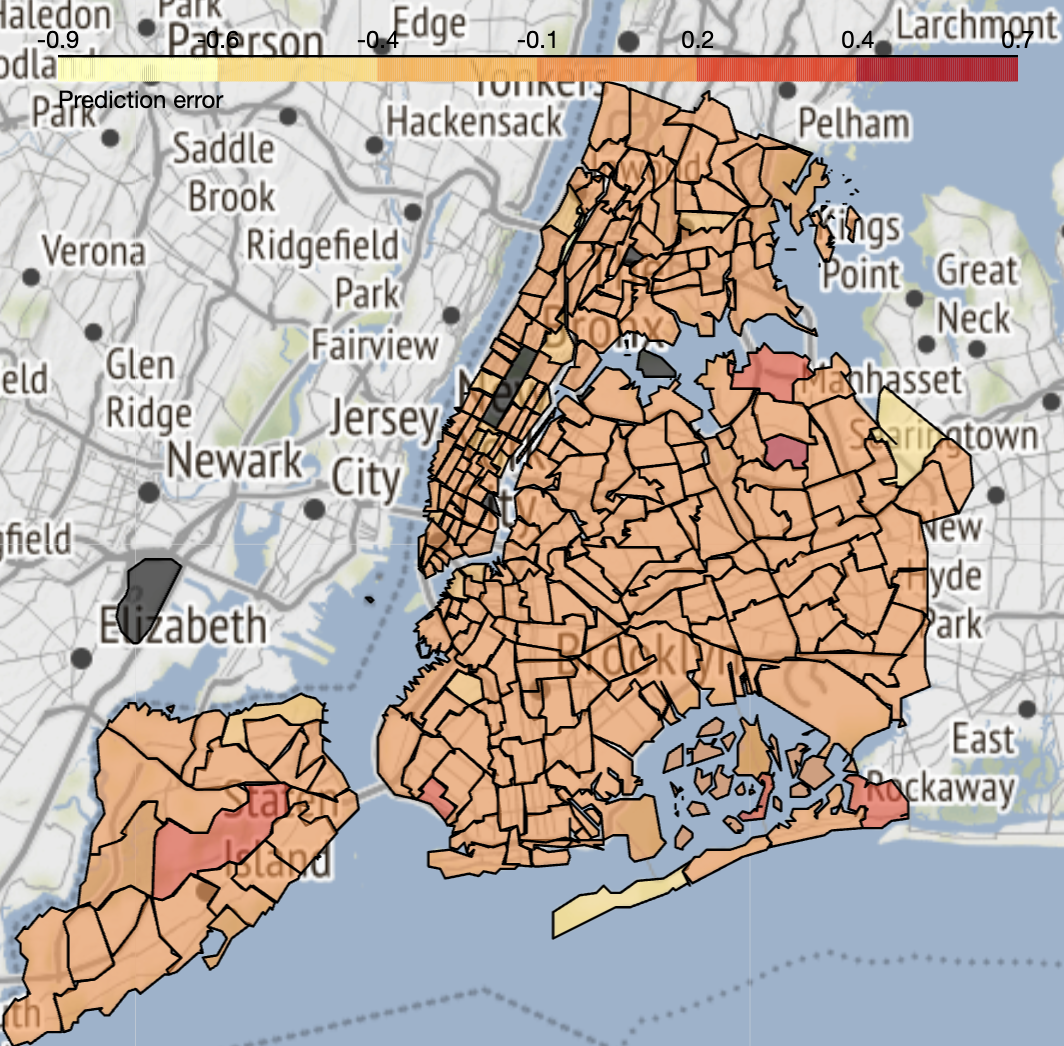
\includegraphics[width=.95\linewidth]{plots/RF_error.png}
        \captionof{figure}{RF prediction error at 6 am}
        \label{RFerror6}
    \end{minipage}
\end{figure}



\section{Recommendations}
From preliminary analysis and model evaluation, conclusion can be drawn that the RF model is  effective in predicting the unit price for FHV in NYC based on only pickup hour, trip time, distance, land use in the area etc. With an RMSE of only 0.0920 on unit price, it can provide FHV drivers with a comprehensive understanding of the dynamic pricing system and a very accurate estimation of earnings to expect.

Drivers are recommended to take advantage of the peak hour in the morning between 5 to 8 am when demand is the highest in NYC. Despite the heavy traffic and possibly severe traffic jam, the unit price is the highest during this time almost everywhere regardless of land use, based on Figure \ref{contrast_loc}. The fare then declines continuously until it reaches the lowest point in the afternoon, hence it is ideal for individual drivers to take some rest in this period. After dinner time, the fare is expected to rise slowly as shown in Figure \ref{PD_one_day}, possibly due to the reduction on the supply side. After midnight, the fare stays high within retail and residential regions, as shown in Figure \ref{contrast_loc}. Drivers, if applicable or determined, can take advantage of this period of time. 

Geographically, Manhattan midtown and downtown have the highest density of non-residential land use. Therefore, the fare in this region is superior to other boroughs during almost any time of the day. Similarly, La Guardia and JFK airports are also hot spots with high unit prices throughout the day, even when other locations experience a trough in price such as 5 pm as shown in Figure \ref{RFpred_17}. On the other hand, most other regions have a relatively lower fare throughout the day. To sum up, drivers are recommended to pick up customers from Manhattan midtown or downtown during the peak hour in the morning, drive to and from the airport during the day and operate between residential and retail areas in the evening and night. 

\begin{figure}[h]
    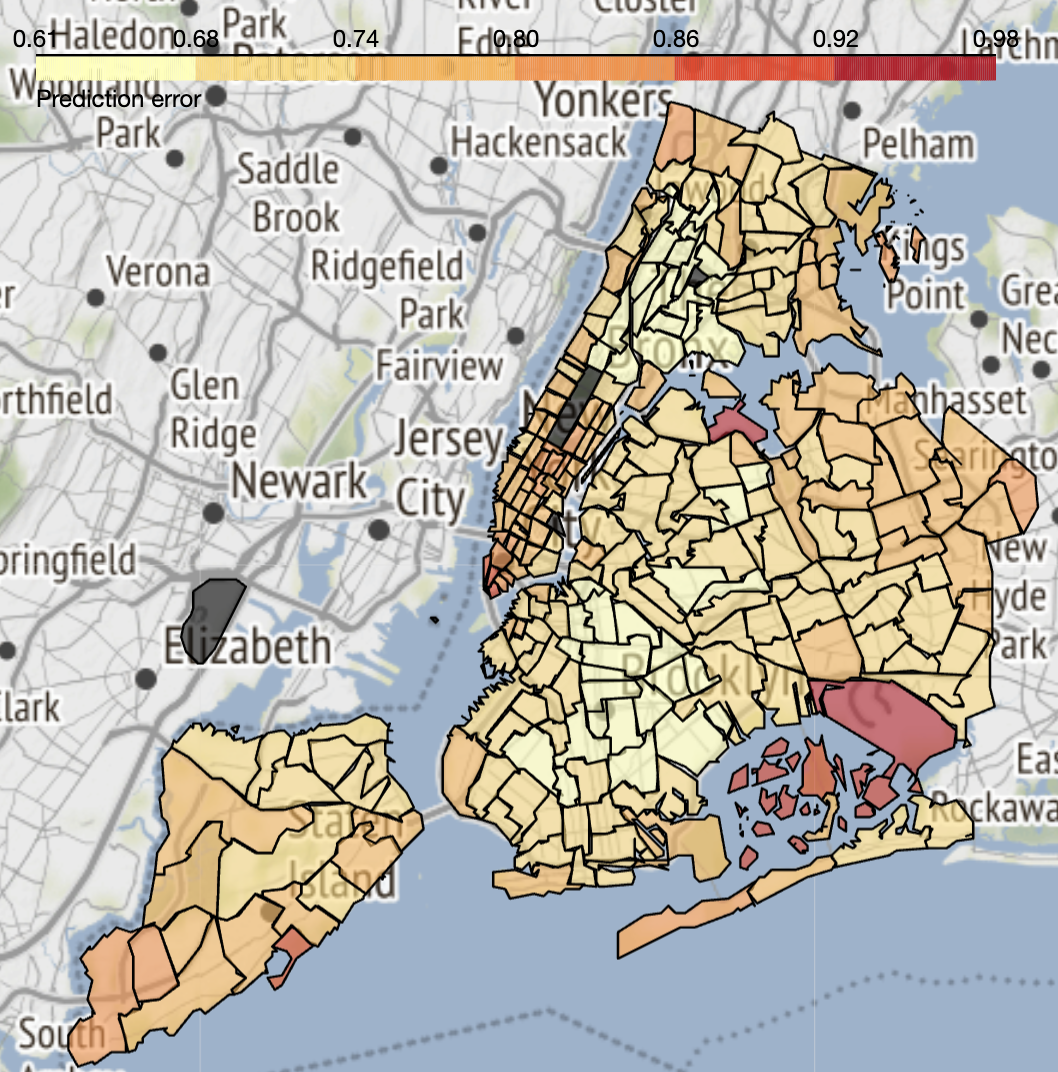
\includegraphics[width=0.5\textwidth]{plots/RFpred_17.png}
    \centering
    \caption{RF prediction of unit price at 5 pm}
    \label{RFpred_17}
\end{figure}

\section{Conclusion}
In this paper, two machine learning models were introduced which were built based on FHV trip records and land use data in NYC for predicting driver's pay per minute at each pickup location during every hour. Both of the models were evaluated and showed promising performance, but the random forest regressor demonstrated better performance. Comprehensive recommendations were made to the target audience - FHV drivers for optimizing their daily routine to maximize earnings. 

Furthermore, the two models and the aggregated dataset used to train them have the potential to explore more complicated problems, such as optimal routing to minimize wait time. Also, the model themselves can be finer-tuned to increase their performance, so that drivers can get a more accurate estimation. 



\clearpage

% BEGIN REFERENCES SECTION
\printbibliography

\end{document}